\section{Experimental Evaluation}
\label{sec:experiment}

In this section, we conduct a practical evaluation through experimentation in 
which we instantiate the semantic models (Figure~\ref{fig:wicusrels}) for three real 
scientific workflow applications. We study and document the Montage~\cite{Montage},
Epigenomics~\cite{genome}, and SoyKB~\cite{soybean, Joshi01012014} workflows 
and their execution environments, which include the application software components 
and the workflow management system.

The goal of this experiment is to reproduce original workflow executions in two different 
Cloud infrastructures, FutureGrid~\cite{futuregrid} and Amazon EC2~\cite{aws}, and a
local execution environment by using Vagrant. 
FutureGrid is an academic Cloud test-bed facility that includes a number of computational 
resources at distributed locations. Amazon Web Services EC2 is a public infrastructure 
provider and the \emph{de facto} standard for IaaS Cloud platforms. 


\subsection{Scientific Workflows}

\paragraph{\textbf{Montage}}
The Montage workflow~\cite{Montage} was created by the NASA Infrared Processing 
and Analysis Center (IPAC) as an open source toolkit that can be used to generate 
custom mosaics of astronomical images in the Flexible Image Transport System (FITS) 
format. In a Montage workflow, the geometry of the output mosaic is calculated from the 
input images. The inputs are then re-projected to have the same spatial scale and rotation, 
the background emissions in the images are corrected to have a uniform level, and the 
re-projected, corrected images are co-added to form the output mosaic. 
Figure~\ref{fig:workflow-montage} illustrates a small (20 node) Montage workflow. The 
size of the workflow depends on the number of images required to construct the desired 
mosaic.

\begin{figure}[!htt]
	\centering
	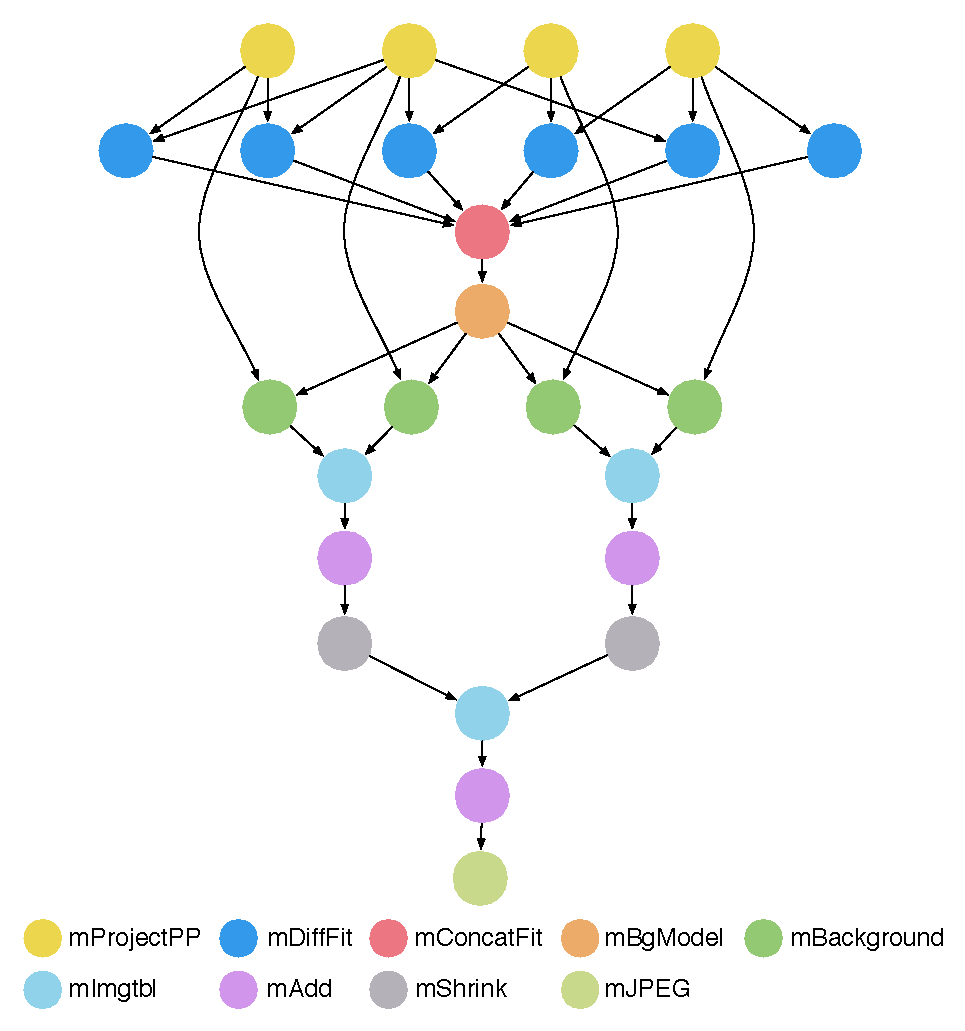
\includegraphics[width=0.9\linewidth]{figures/workflow-montage}
	\caption{A small (20 node) Montage workflow.}
	\label{fig:workflow-montage}
\end{figure}


\paragraph{\textbf{Epigenomics}}
The USC Epigenome Center~\cite{genome} is currently involved in mapping the epigenetic 
state of human cells on a genome-wide scale. The Epigenomics workflow 
(Figure~\ref{fig:workflow-genome}) processes multiple sets of genome sequences in
parallel. These sequences are split into subsets, the subsets are filtered to remove
contaminants, reformatted, then mapped to a reference genome. The mapped sequences are
finally merged and indexed for later analysis. In this work, the Epigenome workflow was 
used to align genome sequence reads to a reference genome for human chromosome 
21. The size of the workflow depends on the chunking factor used on the input data, 
which determines the number of sequence reads in each chunk.

\begin{figure}[!htb]
	\centering
	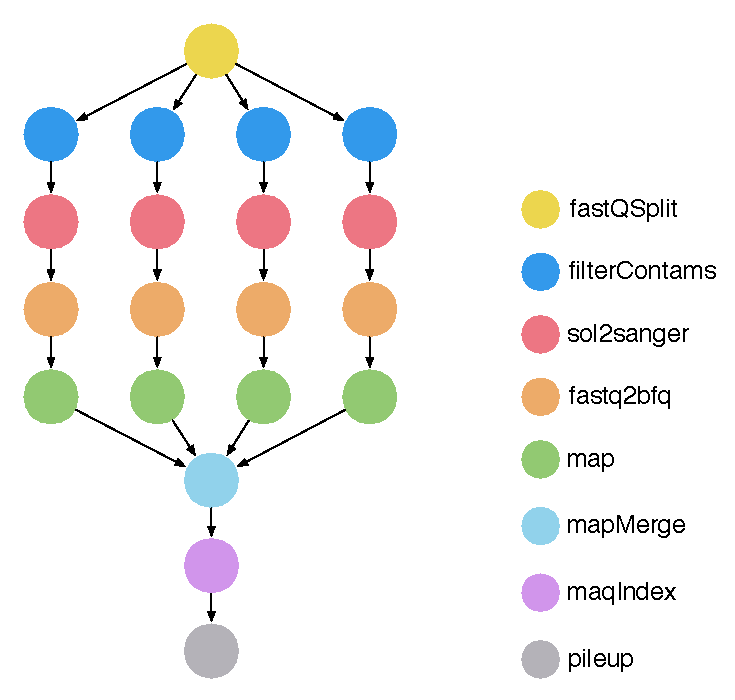
\includegraphics[width=0.75\linewidth]{figures/workflow-genome}
	\caption{Epigenomics workflow.}
	\label{fig:workflow-genome}
\end{figure}

\paragraph{\textbf{SoyKB}}
The SoyKB workflow~\cite{soybean, Joshi01012014} is a genomics pipeline 
that re-sequences soybean germplasm lines selected for desirable traits such 
as oil, protein, soybean cyst nematode resistance, stress resistance, and root 
system architecture. The workflow (Figure~\ref{fig:workflow-soykb}) 
implements a SNP and injection/deletion (indel) identification and analysis 
pipeline using the GATK haplotype caller~\cite{gatk} and a soybean reference 
genome. The workflow analyzes samples in parallel to align them to the reference 
genome, to de-duplicate the data, to identify indels and SNPs, and to merge and 
filter the results. The results are then used for genome-wide association studies 
(GWAS) and genotype to phenotype analysis. The workflow instance used in this 
paper is based on a sample dataset that requires less memory than a full-scale 
production workflow, however it requires the same software components.

\begin{figure}[!htb]
	\centering
	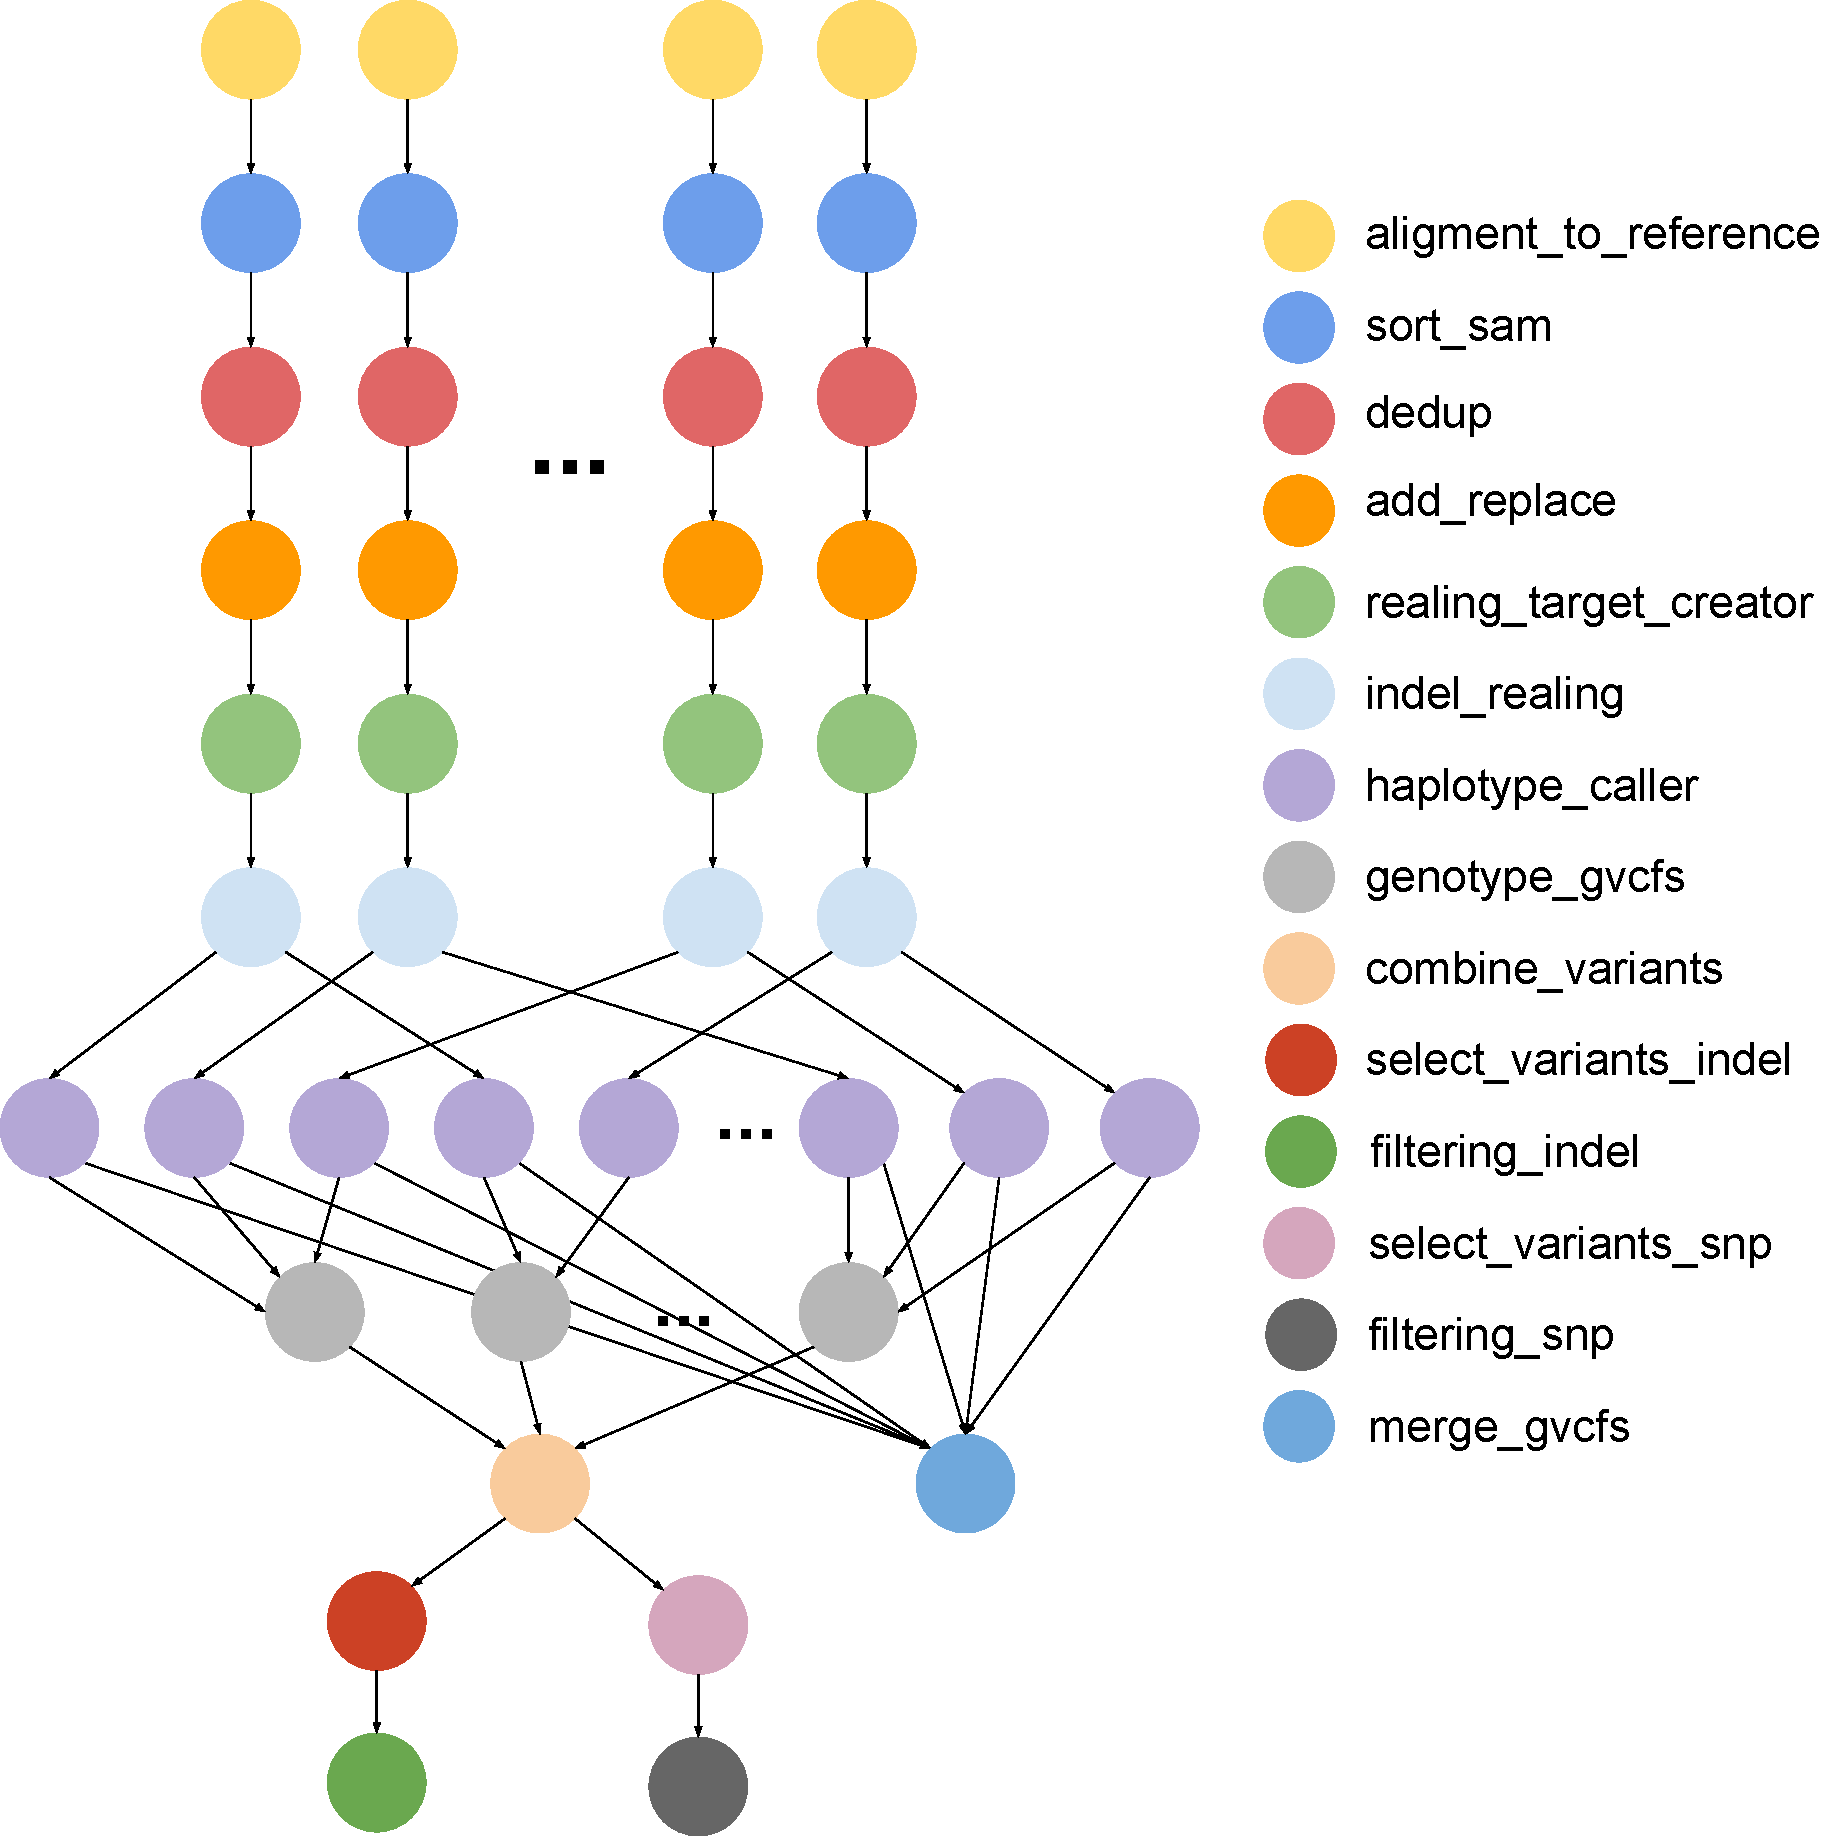
\includegraphics[width=0.95\linewidth]{figures/workflow-soybean}
	\caption{SoyKB workflow.}
	\label{fig:workflow-soykb}
\end{figure}



%%%
\subsection{Generating Semantic Annotations}

In this subsection, we present the annotations generated for each of the scientific 
workflows presented above and the Pegasus WMS using the WICUS ontology
network. As described in Figure~\ref{fig:wicusflow}, the first step in the process of 
documenting a workflow is the annotation of the workflow DAX file. We use the 
\texttt{Workflow} domain ontology to describe a workflow as 1) an individual that 
represents the top level workflow, and 2) a set of individuals representing its 
sub-workflows, one for each transformation. We then generate the necessary 
requirements, one for the top level workflow, which specifies the WMS requirements, 
and one for each sub-workflow, which defines the software components required 
by each transformation. 
Figure~\ref{fig:annotations} shows a simplified overview of the annotations generated 
using the WICUS ontology network for the Montage, Epigenomics, and SoyKB 
workflows as well as for the Pegasus WMS. Below, we describe each of these
semantic annotations in details:

\begin{figure*}[!htb]
	\centering
	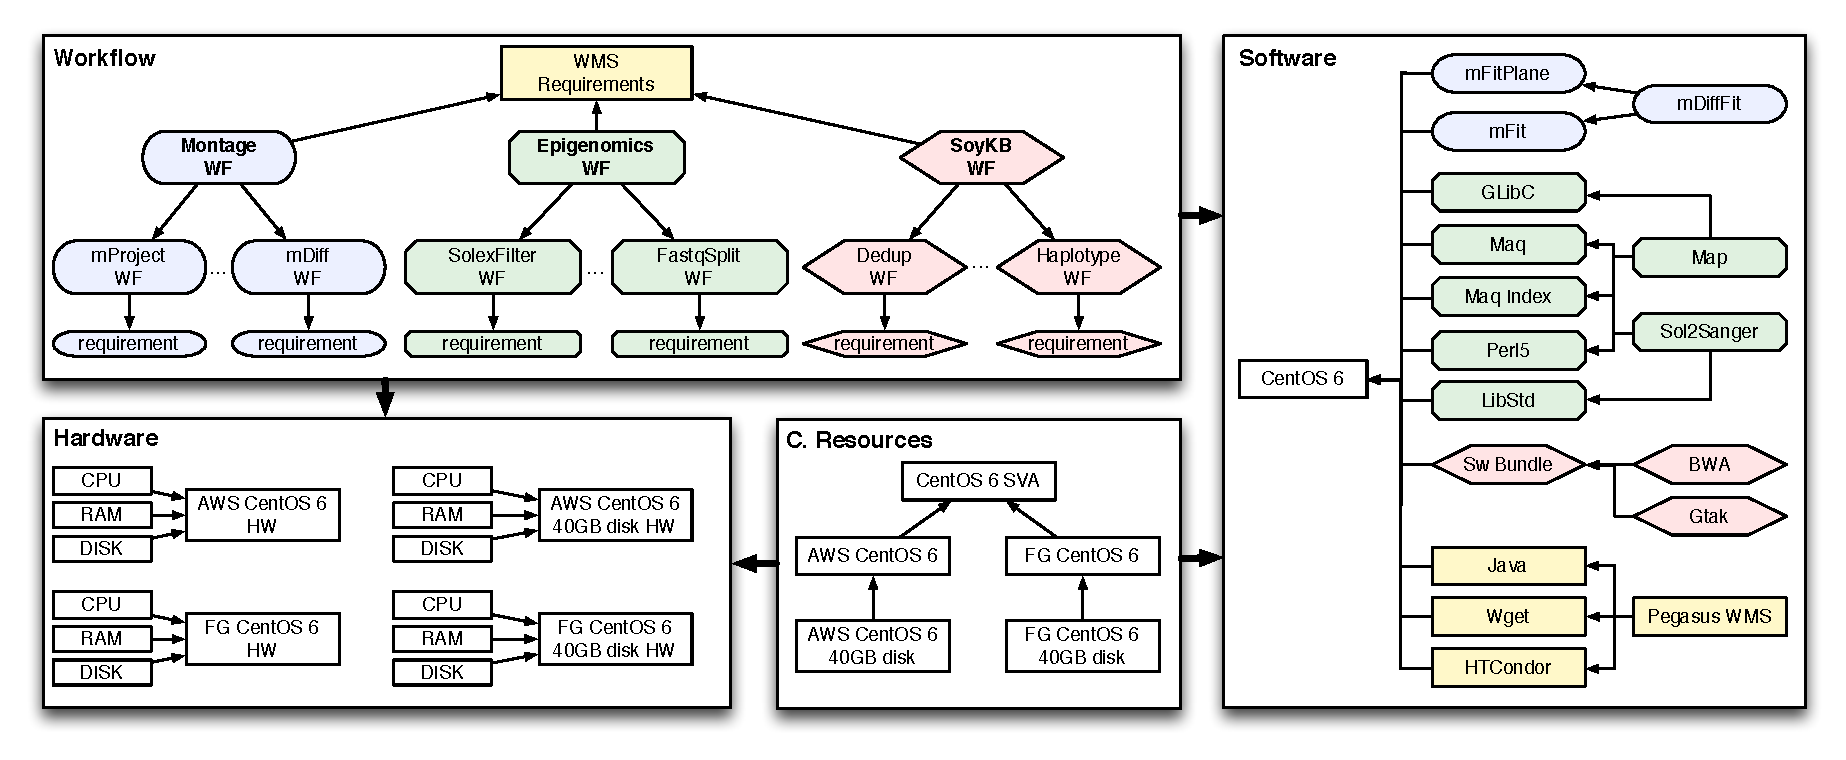
\includegraphics[width=\linewidth]{figures/annotations}
	\vspace{-20pt}
	\caption{Overview of the generated annotations for the Montage, Epigenomics, and 
  	  SoyKB workflows using the WICUS ontology network (yellow rectangles represent the 
	  workflow component; blue squashed rectangles represent the Montage workflow; green 
	  bevelled rectangles represent the Epigenomics workflows; and red hexagons represent 
	  the SoyKB workflow). \note{The figure does not take into account Vagrant.}}
	\label{fig:annotations}
\end{figure*}


\paragraph{\textbf{Workflow Management System}}
We use the \texttt{Software} domain ontology to describe the components that
compose the workflow engine (in this case Pegasus) as individuals, and to 
represent its dependencies. Pegasus relies on \texttt{HTCondor} as task manager, and 
both depend on \texttt{Java} and \texttt{wget}. In addition, all components also
depend on the operating system, which in our case is \texttt{CentOS}. The process
to describe the deployment of the WMS components is based on the installation 
and configuration processes as specified in their documentation. As a result, we 
defined a set of installation scripts for each of the components. These scripts are 
included as part of the deployment plan along with their configuration information.
The WMS components are defined as a requirement (WMS Requirements) using
the \texttt{Workflow} domain ontology. This requirement is then linked to each
of the workflows included in this work. As a result, \texttt{Java}, \texttt{wget}, 
\texttt{HTCondor}, and \texttt{Pegasus WMS} should be installed on the targeted
computational resource.


\paragraph{\textbf{Montage Workflow}}
We use the \texttt{Workflow} domain ontology to describe the Montage workflow 
as an individual that represents the top level workflow, and another 9 individuals 
representing its sub-workflows, one for each transformation. We also generate 9 
requirements, which define the software components required by each transformation. 
At this point, these requirements are empty, as they are not yet related to their 
software components. Figure~\ref{fig:annotations-montage} shows the set of 
generated individuals for the Montage workflow.

\begin{figure}[!htb]
	\centering
	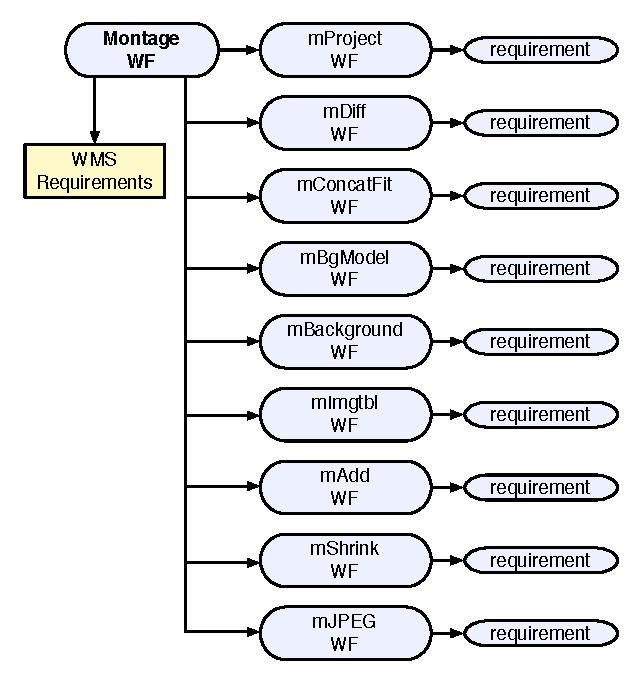
\includegraphics[width=.7\linewidth]{figures/annotations-montage}
	\vspace{-10pt}
	\caption{Annotations for the Montage workflows using the \texttt{Workflow} domain ontology.}
	\label{fig:annotations-montage}
\end{figure}

Application components are described in the Montage workflow's Transformation 
Catalog, where the binary file, version, and destination path are defined. These 
components are also described as individuals using the \texttt{Software} domain 
ontology. We use this information to generate the configuration parameters of the 
deployment script, which in this case is the same for all components. The script 
downloads the binary files from an online repository and copies them to the specified 
destination path. This process identified 59 software components for the Montage 
workflow that are annotated and included in the Software Components Catalog.
Then, the Transformation Catalog Annotator module relates each transformation 
requirement, defined using the \texttt{Workflow} domain ontology, to the application 
component, and therefore to the deployment information. In this experiment, we 
define 9 Montage components that are linked to the requirements, and another two 
sub-components that are defined as dependencies in the software catalog 
(\emph{mDiffFit} depends on the \emph{mDiff} and \emph{mFitPlane} components).


\paragraph{\textbf{Epigenomics Workflow}}
Following the same approach as in the previous case, we use the \texttt{Workflow} 
domain ontology to describe the Epigenomics workflow as an individual that represents 
the top level workflow, and another 8 individuals representing its sub-workflows, one 
for each transformation (Figure~\ref{fig:annotations-genome}). We have then annotated 
the components described in the Epigenomics' Transformation Catalog as individuals 
using the \texttt{Software} domain ontology. We have also identified and annotated 6 
software dependencies related to the workflow, which include the Perl~\cite{perl} interpreter, 
the GNU libc~\cite{libc} and Libstdc++~\cite{libstdc} libraries, and two other binaries from 
the Epigenomics  distribution, \texttt{maq} and \texttt{maqindex}.

\begin{figure}[!htb]
	\centering
	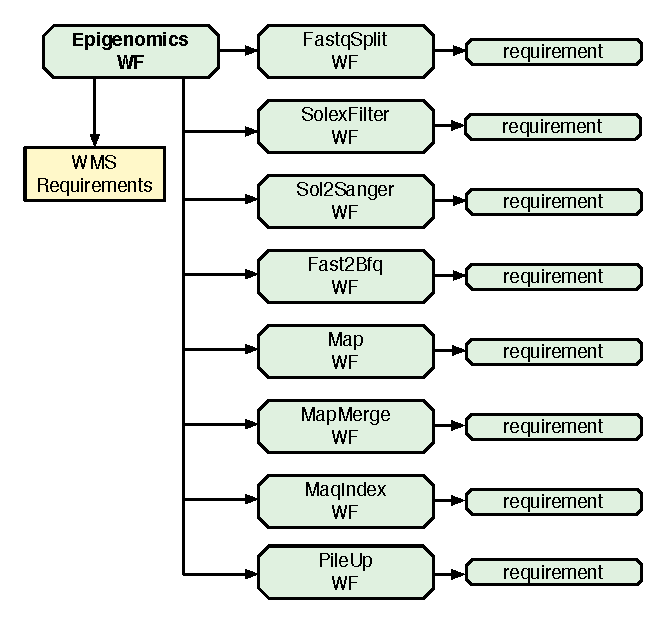
\includegraphics[width=.7\linewidth]{figures/annotations-genome}
	\vspace{-10pt}
	\caption{Annotations for the Epigenomics workflows using the \texttt{Workflow} domain ontology.}
	\label{fig:annotations-genome}
\end{figure}


\paragraph{\textbf{SoyKB Workflow}}
We describe the SoyKB workflow as an individual that represents the top level workflow,
and another 14 individuals representing each transformations. For the sake of simplicity,
we do not show the annotations for this workflow. Although SoyKB is the largest workflow 
in terms of its number of steps (around 670) among the other workflows included in this 
work, it defines only four software components as dependencies (\texttt{bwa-wrapper}, 
\texttt{gatk-wrapper}, \texttt{picard-wrapper}, and \texttt{software-wrapper}). These 
components  are software wrappers that invoke different libraries and binaries depending 
on the parameters used for the execution of the workflow. The components are included 
on a software bundle that is deployed on the computational nodes to be invoked by the 
wrappers. Hence, a dependency for this bundle has been included in the Software 
Components Catalog.


\paragraph{\textbf{Computational Resources}}
We use the \texttt{Computing Resources} and \texttt{Hardware} domain ontologies 
to describe computational resources. For each Cloud resource (Amazon EC2 and 
FutureGrid), we defined two virtual machines: one that meets the requirements for the 
Montage and Epigenomics workflows (requires smaller disk space); and one for the 
SoyKB workflow (requires larger disk space). In both cases, we generated conceptually 
equivalent VMs appliances, as they both provide CentOS 6 operating system, but differed 
in the hardware configuration. We attempt to reduce the resource consumption of
Cloud resources due to the cost for storing/transferring VM images. Since Vagrant
execution is performed locally, we generated a single VM appliance that meets the 
requirements of all workflows. 

The description of the appliances is then included in the Scientific Virtual Appliances 
Catalog (step 7 in Figure~\ref{fig:wicusflow}). We define  an Image Appliance that groups 
all VMs appliances into one single Scientific Virtual Appliance (\texttt{CentOS 6 SVA}). 
Table~\ref{tab:imgapps} summarizes the main characteristics of the five appliances 
we have annotated.

\begin{table}[!htb]
	\centering
	\scriptsize
	\setlength{\tabcolsep}{8pt}
	\begin{tabular}{l | r r | r r | r}
		& \multicolumn{2}{c |}{Amazon EC2} & \multicolumn{2}{c |}{FutureGrid} & \multirow{2}{*}{Vagrant} \\
					& Small & Large & Small & Large \\ \hline
		RAM (GB) 	& 7 &  7 & 8 & 8 &  4 \\
		Disk (GB) 		&  40 &  5 &  40 & 5 & 50 \\
		CPU Freq. (GHz) & 2.4  & 2.4 & 2.9 & 2.9  &  2.7 \\
		CPU Arch. 	& \multicolumn{2}{c|}{64 bits} & \multicolumn{2}{c|}{64 bits} & \multicolumn{1}{c}{64 bits} \\
		OS 			& \multicolumn{2}{c|}{CentOS 6} & \multicolumn{2}{c|}{CentoOS 6} & \multicolumn{1}{c}{CentOS 6} \\
	\end{tabular}
	\caption{CentOS 6 Virtual Image Appliances.}
	\label{tab:imgapps}
\end{table}

\paragraph{\textbf{Hardware Requirements}}

For each of the workflows we have also analyzed which were hardware specifications required for executed them. Table \ref{tab:hwreqs} displays those requirements, describing the minimum threshold for each one of them. During the computational resource selection process we will consider that any machine with equal or higher hardware features than the ones specified will be a valid candidate for running the workflow. In cases such as the CPU frequency, in which we have not identified any specific capacity, we set this value to 0.



\begin{table}[h]
\begin{tabular}{l|llll}
\multicolumn{1}{c|}{} 
 & CPU (GHz) & CPU arch & RAM (GB) & DISK (GB) \\ \hline
Montage &  0 &  64 & 4 & 4 \\ \hline
Epigenomics &  0 &  64 &  4 & 4  \\ \hline
SoyKB & 0  & 64 & 4 & 10  \\ \hline
\end{tabular}
\caption{Workflow hardware requirements}
\label{tab:hwreqs}
\note{Idafen, improve the format of the table}
\end{table}


%%%
\subsection{Reproducing Workflow Executions.}

The last step on the process for achieving reproducibility in scientific workflows (Figure~\ref{fig:wicusflow}) is to execute the Infrastructure Specification Algorithm (ISA). The ISA combines the annotated data based on the 4 domain ontologies in order to find a suitable infrastructure specification that is able to run the workflow. The algorithm retrieves and propagates the WMS requirements of the top-level workflow (\texttt{Workflow} domain ontology) to its related sub-workflows. Requirements and software components are matched, and a dependency graph is built based on the relation between the requirements and the component dependencies. This graph is then used to compute the intersection between the set of software components from the SVA and the dependency graph of each sub-workflow. ISA selects the intersection where the value is maximized for each sub-workflow. Software components already available in the SVA are then removed from the chosen graph. To reduce the number of SVAs, the algorithm attempts to merge sub-workflows requirements into a single SVA. Requirements can be merged if all their software components are compatible. ISA also filters all those Image Appliances, belonging to the selected SVAs, that do not meet the hardware requirements specified for the workflow. Finally, ISA generates a script (either using PRECIP or Vagrant) with the set of required instructions to instantiate, configure, and deploy the computational resources and software components on the corresponding provider.

As introduced in~\cite{wicus} the ISA retrieves the corresponding information for the workflow and its dependencies from the annotations datasets. It calculates the dependencies and the compatibility between requirements and the available computational resources. It also takes into account the already installed software to avoid the unnecessary installation of components.

For this work we have added two main new features to the ISA. First of all we are now able to filter those Image Appliances that do not meet the hardware requirements specified for the target workflow (lines 25-27). Secondly have improved the script generation process, so we are now able to also generate Vagrant scripts. For this process we first generate an abstract deployment plan, defining the steps and scripts to be executed, along with their configuration parameters. The ISA then concretizes this plan into a PRECIP or Vagrant script depending on the resultant target provider (line 29).

A pseudo-code overview of the main steps of the ISA is listed in Listing \ref{lst:pseudo}.

\lstset{language=C++,
	  numbers=left,
	   numberstyle=\tiny\color{mygray},
           basicstyle=\ttfamily\scriptsize,
          breaklines=true,
          }
          
\begin{lstlisting}[caption={Pseudo-code overview of the ISA},label={lst:pseudo}]
WorkflowRequirementsDataset.load();

SVADataset.load();

SoftwareCatalogDataset.load();

Map<Workflow,List<Requirements>> wfSwReqs = 
  retrieveSwRequirements(WorkflowRequirementsDataset, WorkflowID);

Map<Workflow,List<Requirements>> propagatedWfSwReqs = 
  propagateSwReqs(wfSwReqs);

List<List<List<SWComponents>>> softwareComponents = getSoftwareComponents(propagatedWfSwReqs);

Map<Requirement,D-Graph<SWComponents>> softwareComponentsDependencyGraph = getSoftwareDependencies(softwareComponents);

List<SVA> availableSvas = getAvailableSvas(providersList);

Map<Requirements,SVA> maxCompatibilities = getCompatibilityIntersection(softwareComponentsDependencyGraph,availableSvas);

Map<Requirement,D-Graph<SWComponents>> substractedSwComponentsDepGraph = substractSoftwareComponents(softwareComponentsDependencyGraph, maxCompatibilities);

Map<SVA, List<Requirments>>mergedSvas= mergeSubworkflows(propagatedWfSwReqs, maxCompatibilities);

Map<Workflow,List<Requirements>> wfHwReqs =   retrieveHwRequirements(WorkflowRequirementsDataset, WorkflowID);

Map<SVA, List<Requirments>>filteredSvas= getCompatibleHwImageAppliances(mergedSvas,wfHwReqs);

generateScript(filteredSvas ,substractedSwComponentsDepGraph);

\end{lstlisting}


In this experiment, we execute ISA over the annotated data specifying the three different providers we work with. As result we obtain the abstract plans listed in listings \ref{lst:plan-montge}, \ref{lst:plan-epigenomics}, and \ref{lst:plan-soykb}. 


\note{Idafen, add diagram defining how STACK, COMP, PLAN, and STEP are related}
\note{Idafen, use only one listing (soykb) and explain it main parts}


\begin{lstlisting}[caption={Abstract deployment plan of the Montage WF},label={lst:plan-montge}]
OPEN_SSH_CLIENTS_SOFT_STACK stack
 OPEN_SSH_CLIENTS_SOFT_COMP component
  OPEN_SSH_CLIENTS_DEP_STEP step
OPEN_SSH_SERVER_SOFT_STACK stack
 OPEN_SSH_SERVER_SOFT_COMP component
  OPEN_SSH_SERVER_DEP_STEP step
WGET_SOFT_STACK stack
 WGET_SOFT_COMP component
  WGET_DEP_STEP step
CONDOR_CENTOS_6_5_SOFT_STACK stack
 CONDOR_CENTOS_6_5_SOFT_COMP component
  STOP_CONDOR_DEP_STEP step
  ADD_CONDOR_REPO_DEP_STEP step
  CONDOR_YUM_INSTALL_DEP_STEP step
  CLEAN_AND_SET_CONDOR_DEP_STEP step
  RESTART_DAEMONS_DEP_STEP step
JAVA-1.7.0-OPENJDK.X86_64_SOFT_STACK stack
 JAVA-1.7.0-OPENJDK.X86_64_SOFT_COMP component
  JAVA-1.7.0-OPENJDK.X86_64_DEP_STEP step
JAVA-1.7.0-OPENJDK-DEVEL.X86_64_SOFT_STACK stack
 JAVA-1.7.0-OPENJDK-DEVEL.X86_64_SOFT_COMP component
  JAVA-1.7.0-OPENJDK-DEVEL.X86_64_DEP_STEP step
PEGASUS_WMS_CENTOS_6_5_SOFT_STACK stack
 PEGASUS_WMS_CENTOS_6_5_SOFT_COMP component
  ADD_PEGASUS_REPO_DEP_STEP step
  PEGASUS_YUM_INSTALL_DEP_STEP step
MFITPLANE_SOFT_STACK stack
 MFITPLANE_SOFT_COMP component
  MFITPLANE_DEP_STEP step
MDIFF_SOFT_STACK stack
 MDIFF_SOFT_COMP component
  MDIFF_DEP_STEP step
MDIFFFIT_SOFT_STACK stack
 MDIFFFIT_SOFT_COMP component
  MDIFFFIT_DEP_STEP step
MCONCATFIT_SOFT_STACK stack
 MCONCATFIT_SOFT_COMP component
  MCONCATFIT_DEP_STEP step
MIMGTBL_SOFT_STACK stack
 MIMGTBL_SOFT_COMP component
  MIMGTBL_DEP_STEP step
MSHRINK_SOFT_STACK stack
 MSHRINK_SOFT_COMP component
  MSHRINK_DEP_STEP step
MPROJECTPP_SOFT_STACK stack
 MPROJECTPP_SOFT_COMP component
  MPROJECTPP_DEP_STEP step
MADD_SOFT_STACK stack
 MADD_SOFT_COMP component
  MADD_DEP_STEP step
MBACKGROUND_SOFT_STACK stack
 MBACKGROUND_SOFT_COMP component
  MBACKGROUND_DEP_STEP step
MBGMODEL_SOFT_STACK stack
 MBGMODEL_SOFT_COMP component
  MBGMODEL_DEP_STEP step
MJPEG_SOFT_STACK stack
 MJPEG_SOFT_COMP component
  MJPEG_DEP_STEP step
\end{lstlisting}


\begin{lstlisting}[caption={Abstract deployment plan of the Epigenomics WF},label={lst:plan-epigenomics}]
OPEN_SSH_CLIENTS_SOFT_STACK stack
 OPEN_SSH_CLIENTS_SOFT_COMP component
  OPEN_SSH_CLIENTS_DEP_STEP step
OPEN_SSH_SERVER_SOFT_STACK stack
 OPEN_SSH_SERVER_SOFT_COMP component
  OPEN_SSH_SERVER_DEP_STEP step
WGET_SOFT_STACK stack
 WGET_SOFT_COMP component
  WGET_DEP_STEP step
CONDOR_CENTOS_6_5_SOFT_STACK stack
 CONDOR_CENTOS_6_5_SOFT_COMP component
  STOP_CONDOR_DEP_STEP step
  ADD_CONDOR_REPO_DEP_STEP step
  CONDOR_YUM_INSTALL_DEP_STEP step
  CLEAN_AND_SET_CONDOR_DEP_STEP step
  RESTART_DAEMONS_DEP_STEP step
JAVA-1.7.0-OPENJDK.X86_64_SOFT_STACK stack
 JAVA-1.7.0-OPENJDK.X86_64_SOFT_COMP component
  JAVA-1.7.0-OPENJDK.X86_64_DEP_STEP step
JAVA-1.7.0-OPENJDK-DEVEL.X86_64_SOFT_STACK stack
 JAVA-1.7.0-OPENJDK-DEVEL.X86_64_SOFT_COMP component
  JAVA-1.7.0-OPENJDK-DEVEL.X86_64_DEP_STEP step
PEGASUS_WMS_CENTOS_6_5_SOFT_STACK stack
 PEGASUS_WMS_CENTOS_6_5_SOFT_COMP component
  ADD_PEGASUS_REPO_DEP_STEP step
  PEGASUS_YUM_INSTALL_DEP_STEP step
MAQ_INDEX_X86_64_SOFT_STACK stack
 MAQ_INDEX_X86_64_SOFT_COMP component (version: 1.0)
  MAQ_INDEX_X86_64_DEP_STEP step
  MAQ_INDEX_X86_64_2_DEP_STEP step
MAQ_X86_64_SOFT_STACK stack
 MAQ_X86_64_SOFT_COMP component (version: 1.0)
  MAQ_X86_64_DEP_STEP step
  MAQ_X86_64_2_DEP_STEP step
RPM_GLIBCi686_SOFT_STACK stack
 RPM_GLIBCi686_SOFT_COMP component
  RPM_GLIBCi686_DEP_STEP step
RPM_GLIBC_X86_64_SOFT_STACK stack
 RPM_GLIBC_X86_64_SOFT_COMP component
  RPM_GLIBC_X86_64_DEP_STEP step
RPM_COMPAT_LIBSTDCPP_33_X86_64_SOFT_STACK stack
 RPM_COMPAT_LIBSTDCPP_33_X86_64_SOFT_COMP component
  RPM_COMPAT_LIBSTDCPP_33_X86_64_DEP_STEP step
RPM_PERL_V5_14_4_X86_64_SOFT_STACK stack
 RPM_PERL_V5_14_4_X86_64_SOFT_COMP component
  RPM_PERL_V5_14_4_X86_64_DEP_STEP step
FASTQSPLIT_SOFT_STACK stack
 FASTQSPLIT_SOFT_COMP component (version: 1.0)
  FASTQSPLIT_DEP_STEP step
  FASTQSPLIT_2_DEP_STEP step
SOL2SANGER_SOFT_STACK stack
 SOL2SANGER_SOFT_COMP component (version: 1.0)
  SOL2SANGER_DEP_STEP step
  SOL2SANGER_2_DEP_STEP step
MAP_SOFT_STACK stack
 MAP_SOFT_COMP component (version: 1.0)
  MAP_DEP_STEP step
  MAP_2_DEP_STEP step
CHR21_SOFT_STACK stack
 CHR21_SOFT_COMP component (version: 1.0)
  CHR21_DEP_STEP step
  CHR21_2_DEP_STEP step
PILEUP_SOFT_STACK stack
 PILEUP_SOFT_COMP component (version: 1.0)
  PILEUP_DEP_STEP step
  PILEUP_2_DEP_STEP step
FAST2BFQ_SOFT_STACK stack
 FAST2BFQ_SOFT_COMP component (version: 1.0)
  FAST2BFQ_DEP_STEP step
  FAST2BFQ_2_DEP_STEP step
MAPMERGE_SOFT_STACK stack
 MAPMERGE_SOFT_COMP component (version: 1.0)
  MAPMERGE_DEP_STEP step
  MAPMERGE_2_DEP_STEP step
FILTERCONTAMS_SOFT_STACK stack
 FILTERCONTAMS_SOFT_COMP component (version: 1.0)
  FILTERCONTAMS_DEP_STEP step
  FILTERCONTAMS_2_DEP_STEP step
\end{lstlisting}


\begin{lstlisting}[caption={Abstract deployment plan of the SoyKB WF},label={lst:plan-soykb}]
  OPEN_SSH_CLIENTS_SOFT_STACK stack
   OPEN_SSH_CLIENTS_SOFT_COMP component
    OPEN_SSH_CLIENTS_DEP_STEP step
  OPEN_SSH_SERVER_SOFT_STACK stack
   OPEN_SSH_SERVER_SOFT_COMP component
    OPEN_SSH_SERVER_DEP_STEP step
  WGET_SOFT_STACK stack
   WGET_SOFT_COMP component
    WGET_DEP_STEP step
  CONDOR_CENTOS_6_5_SOFT_STACK stack
   CONDOR_CENTOS_6_5_SOFT_COMP component
    STOP_CONDOR_DEP_STEP step
    ADD_CONDOR_REPO_DEP_STEP step
    CONDOR_YUM_INSTALL_DEP_STEP step
    CLEAN_AND_SET_CONDOR_DEP_STEP step
    RESTART_DAEMONS_DEP_STEP step
  JAVA-1.7.0-OPENJDK.X86_64_SOFT_STACK stack
   JAVA-1.7.0-OPENJDK.X86_64_SOFT_COMP component
    JAVA-1.7.0-OPENJDK.X86_64_DEP_STEP step
  JAVA-1.7.0-OPENJDK-DEVEL.X86_64_SOFT_STACK stack
   JAVA-1.7.0-OPENJDK-DEVEL.X86_64_SOFT_COMP component
    JAVA-1.7.0-OPENJDK-DEVEL.X86_64_DEP_STEP step
  PEGASUS_WMS_CENTOS_6_5_SOFT_STACK stack
   PEGASUS_WMS_CENTOS_6_5_SOFT_COMP component
    ADD_PEGASUS_REPO_DEP_STEP step
    PEGASUS_YUM_INSTALL_DEP_STEP step
  SOFTWARE_TAR_GZ_SOFT_STACK stack
   SOFTWARE_TAR_GZ_SOFT_COMP component
    SOFTWARE_TAR_GZ_DEP_STEP step
  PICARD-WRAPPER_SOFT_STACK stack
   PICARD-WRAPPER_SOFT_COMP component
    PICARD-WRAPPER_DEP_STEP step
    PICARD-WRAPPER_2_DEP_STEP step
  SOFTWARE-WRAPPER_SOFT_STACK stack
   SOFTWARE-WRAPPER_SOFT_COMP component
    SOFTWARE-WRAPPER_DEP_STEP step
    SOFTWARE-WRAPPER_2_DEP_STEP step
  GATK-WRAPPER_SOFT_STACK stack
   GATK-WRAPPER_SOFT_COMP component
    GATK-WRAPPER_DEP_STEP step
    GATK-WRAPPER_2_DEP_STEP step
  BWA-WRAPPER_SOFT_STACK stack
   BWA-WRAPPER_SOFT_COMP component
    BWA-WRAPPER_DEP_STEP step
    BWA-WRAPPER_2_DEP_STEP step
\end{lstlisting}

In all cases, the algorithm is able to concretize the abstract plan either to a PRECIP or a Vagrant script (depending on the specified provider). Each generated script is composed by the following main sections:

\begin{itemize}

	\item \emph{Experiment Creation}: generates a new experiment using the given VM image ID and the user credentials for the selected infrastructure provider;
    	    
	\item \emph{Software Deployment}: executes the set of instructions defined on the deployment plan of each software component to install and configure the required software to execute the workflow. In this section, both the workflow management system and the application are deployed with their dependencies;

	\item \emph{User Setup}: creates a user account on the VM (if it does not exist) and configures the necessary SSH keys to enable file transfers and execution. This account will be used to run the workflow;
	   
	\item \emph{Data Stage and Workflow Execution}: stages all the input data of the Montage workflow on the VM, and launches the workflow execution. Since our work is focused on infrastructure reproducibility, data and workflow management are not covered in our approach.

\end{itemize}

\noindent Note that all the configuration and deployment commands (first 3 sections) require superuser privileges on the VM. The workflow execution, however, is performed under the user account created in the third section.


\note{Idafen, modify this including the results of the 3 WFs, and how we check results are correct}.

We executed the scripts on their corresponding platforms. Both executions succeeded on deploying and running the Montage workflow, the Pegasus WMS, and their dependencies. We also performed the same execution of the Montage workflow in a predefined VM image, where the execution environment is already in place. Results show that the VM execution environments deployed by both scripts are equivalent to the former one. In addition, we used a perceptual hash tool\footnote{pHash - \url{http://www.phash.org}} to compare the resulting image (0.1 degree image of the sky) generated by both executions against the one generated by the baseline execution. We obtained a similarity factor of 1.0 (over 1.0) with a threshold of 0.85, which means the images are identical. Therefore we are obtaining the same results as the original workflow. In this work we do not aim to reproduce either the performance or the execution time of the original experiment.



All the original and generated scripts are available as part of the experimental material included in the Research Object (RO)~\cite{researchObjects} associated with this paper\footnote{\url{http://pegasus.isi.edu/publications/FGCS(CREATE-RO!)}}. This RO also contains pointers to the software and resources used in this experiment.